\documentclass[a4paper,11pt]{article}

\usepackage[utf8x]{inputenc}
\usepackage[british]{babel}

\usepackage{amsmath, amsfonts, amssymb, amsthm, amscd}
\usepackage{listings}
\usepackage{courier}

\usepackage{graphicx}

\lstset{
  language=C,
  basicstyle=\ttfamily,
%  keywordstyle=\ttfamily,
  frame=none,
  captionpos=b,
  mathescape=true,
  morekeywords={alignof, sizeType, promote, bool, restrict, memcpy, memmove},
  % escapeinside={\%*}{*)}
}

\title{Effective Types}
\date{10th October 2012}

\begin{document}
\maketitle

\section{Definition}
Effective types have been introduced to allow compilers to infer aliasing
information from types. If two pointers have incompatible types, then a
compiler should be allowed to assume that memory accesses through these
pointers do not touch the same chunk of memory. As a reminder, the two
fundamental rules are (c.f. section 6.5):
\begin{quote}
  \begin{enumerate}
  \item[6]
    The {\em effective type} of an object for an access to its stored value
    is the declared type of the object, if any.$^{87)}$ If a value is stored
    into an object having no declared type through an lvalue having a type
    that is not a character type, then the type of the lvalue becomes the
    effective type of the object for that access and for subsequent accesses
    that do not modify the stored value. If a value is copied into an object
    having no declared type using {\lstinline {memcpy}} or {\lstinline
      {memmove}}, or is copied as an array of character type, then the
    effective type of the modified object for that access and for subsequent
    accesses that do not modify the value is the effective type of the
    object from which the value is copied, if it has one. For all other
    accesses to an object having no declared type, the effective type of the
    object is simply the type of the lvalue used for the
    access.
  \item[7]
    An object shall have its stored value accessed only by an lvalue
    expression that has one of the following types:$^{88)}$

    \begin{itemize}
      \item[---] a type compatible with the effective type of the object,
      \item[---] ...
    \end{itemize}
  \end{enumerate}

  \hrulefill\\
  {\footnotesize
    \begin{enumerate}
    \item[87)] Allocated objects have no declared type.
    \item[88)] The intent of this list is to specify those circumstances in
      which an object may or may not be aliased.
    \end{enumerate}
  }
\end{quote}

\section{Issue}

\begin{figure}[h]
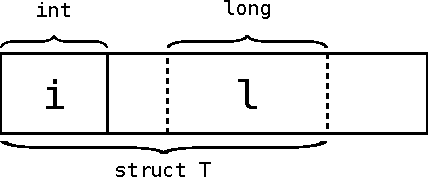
\includegraphics{pictures/malloc-T}
\centering
\end{figure}


\begin{lstlisting}
struct T {
  int  i;
  long l;
};

T *p = malloc(sizeof(T));
assert (p != NULL);

p->i = 1;
p->l = 0;
printf("%d\n", p.i);
\end{lstlisting}

\section{Idea}
The pointer \lstinline{p->i}  {\em pointer to object of type \lstinline{int}}
but instead it will be given a fancier type that keeps track of the
structure/array context of sub-objects, e.g.   {\em pointer to field \lstinline{m} inside a structure of type \lstinline{T}}

semantics value was just a (unique) symbolic name

\section{Implementation}

\end{document}

%%% Local Variables: 
%%% mode: latex
%%% TeX-master: t
%%% End: 
